%!TEX root =../../course-notes.tex
% ^ leave for LaTeXTools build functionality

\begin{applicationActivities}{1}{25}

\begin{activity}{5}
The image below illustrates how the linear transformation
$T_1 : \IR^2 \rightarrow \IR^2$ given by the
standard matrix $A_1 = \begin{bmatrix} 2 & 0 \\ 0 & 3 \end{bmatrix}$
transforms the unit square.

\begin{center}
\begin{tikzpicture}[scale=0.5]
\draw[thin,gray,<->] (-4,0)-- (4,0);
\draw[thin,gray,<->] (0,-4)-- (0,4);
\draw[thick,blue,->] (0,0) -- node[below] {$A_1 \vec{e}_1= \begin{bmatrix}2 \\ 0 \end{bmatrix}$}++ (2,0);
\draw[thick,blue,->] (0,0) -- node[left] {$A_1 \vec{e}_2 = \begin{bmatrix} 0 \\ 3 \end{bmatrix}$}++(0,3);
\draw[thick,dashed,red,->] (0,0) -- ++(1,0);
\draw[thick,dashed,red,->] (0,0) -- ++(0,1);
\draw[blue,dashed] (2,0) -- (2,3) -- (0,3);
\draw[red,dashed] (1,0) -- (1,1) -- (0,1);
\end{tikzpicture}
\end{center}

\begin{enumerate}[(a)]
\item What is the area of the transformed unit square?
\item Find two vectors that were stretched/compressed by the
      transformation (not sheared),
      and compute how much those vectors were stretched/compressed.
\end{enumerate}

\end{activity}


\begin{activity}{5}
The image below illustrates how the linear transformation
$T_2 : \IR^2 \rightarrow \IR^2$ given by the
standard matrix $A_2 = \begin{bmatrix} 3 & 3 \\ 0 & 2 \end{bmatrix}$.
transforms the unit square.

\begin{center}
\begin{tikzpicture}[scale=0.5]
\draw[thin,gray,<->] (-4,0)-- (4,0);
\draw[thin,gray,<->] (0,-4)-- (0,4);
\draw[thick,blue,->] (0,0) -- node[below] {$A_2 \vec{e}_1= \begin{bmatrix}3 \\ 0 \end{bmatrix}$}++ (3,0);
\draw[thick,blue,->] (0,0) -- ++(3,2) node[above] {$A_2 \vec{e}_2 = \begin{bmatrix} 3 \\ 2 \end{bmatrix}$};
\draw[thick,dashed,red,->] (0,0) -- ++(1,0);
\draw[thick,dashed,red,->] (0,0) -- ++(0,1);
\draw[blue,dashed] (3,0) -- (6,2) -- (3,2);
\draw[red,dashed] (1,0) -- (1,1) -- (0,1);
\end{tikzpicture}
\end{center}

\begin{enumerate}[(a)]
\item What is the area of the transformed unit square?
\item Find at least one vector that was stretched/compressed by the
      transformation (not sheared),
      and compute how much those vectors were stretched/compressed.
\end{enumerate}
\end{activity}

\begin{observation}
  It's possible to find two non-parallel vectors that are stretched by the
  transformation given by \(A_2\):
  % \(A_2\begin{bmatrix}1\\0\end{bmatrix}=3\begin{bmatrix}1\\0\end{bmatrix}\)
  % and
  % \(A_2\begin{bmatrix}-1\\1/3\end{bmatrix}=2\begin{bmatrix}-1\\1/3\end{bmatrix}\)

  \begin{center}
  \begin{tikzpicture}[scale=0.5]
  \draw[thin,gray,<->] (-4,0)-- (4,0);
  \draw[thin,gray,<->] (0,-4)-- (0,4);
  \draw[thick,blue,->] (0,0) -- node[below] {$A_2\begin{bmatrix}1\\0\end{bmatrix}=3\begin{bmatrix}1\\0\end{bmatrix}$}++ (3,0);
  \draw[thick,blue,->] (0,0) -- ++(-2,0.67) node[above] {$A_2\begin{bmatrix}-1\\1/3\end{bmatrix}=2\begin{bmatrix}-1\\1/3\end{bmatrix}$};
  \draw[thick,red,->] (0,0) -- (1,0);
  \draw[thick,red,->] (0,0) -- (-1,0.33);
  \end{tikzpicture}
  \end{center}

  The process for finding such vectors will be covered later in this module.
\end{observation}


\begin{activity}{5}
Consider the linear transformation given by the standard matrix
 $A_3 = \begin{bmatrix} 1 & -1 \\ 1 & 1 \end{bmatrix}$.

\begin{enumerate}[(a)]
\item Sketch the transformation of the unit square
      (the parallelogram given by the columns of the standard matrix).
\item Compute the area of the transformed unit square.
\end{enumerate}
\end{activity}


\begin{activity}{5}
Consider the linear transformation given by the standard matrix
 $A_4 = \begin{bmatrix} 0 & 1 \\ 1 & 0 \end{bmatrix}$.

\begin{enumerate}[(a)]
\item Sketch the transformation of the unit square.
\item Compute the area of the transformed unit square.
\end{enumerate}
\end{activity}

\begin{activity}{5}
Consider the linear transformation given by the standard matrix
 $A_5 = \begin{bmatrix} 1 & 1 \\ 0 & 0 \end{bmatrix}$.

\begin{enumerate}[(a)]
\item Sketch the transformation of the unit square.
\item Compute the area of the transformed unit square.
\end{enumerate}
\end{activity}


\begin{remark}
The area of the transformed unit square measures the factor by which
all areas are transformed by a linear transformation.

We will define the \term{determinant} of a square matrix \(A\),
or \(\det(A)\) for short, to be this factor. But
what properties must this function satisfy?
\end{remark}

% \begin{activity}{5}
% Label each of the four pictures with the most appropriate of the
% following four expressions.
%
% \begin{center}
% \begin{minipage}{0.8\textwidth}
% \begin{align*}
% \det([\vec{e}_1\,\vec{e}_2]) &&
% \det([\vec{v}\,\vec{v}]) &&
% \det([c\vec{v}\,\vec{w}])  &&
% \det([\vec{u}+\vec{v}\,\vec{w}])
% \end{align*}
%
%
% \begin{multicols}{2}
% \begin{center}
% \begin{tikzpicture}[scale=0.8]
% \draw[thin,gray,<->] (-1,0)-- (3,0);
% \draw[thin,gray,<->] (0,-1)-- (0,3);
% \draw[thick,blue,->] (0,0) -- node[below] {$\vec{e}_1$} (1,0);
% \draw[thick,blue,->] (0,0) -- node[left] {$\vec{e}_2$} (0,1);
% \draw[thick,blue,->] (1,0) -- (1,1);
% \draw[thick,blue,->] (0,1) -- (1,1);
% \end{tikzpicture}
% \end{center}
%
% \begin{center}
% \begin{tikzpicture}[scale=0.5]
% \draw[thin,gray,<->] (-1,0)-- (4,0);
% \draw[thin,gray,<->] (0,-1)-- (0,4);
% \draw[thick,blue,->] (0,0) -- node[below] {$\vec{v}$} (3,2);
% \end{tikzpicture}
% \end{center}
%
%
% \begin{center}
% \begin{tikzpicture}[scale=0.5]
% \draw[thin,gray,<->] (-1,0)-- (6,0);
% \draw[thin,gray,<->] (0,-1)-- (0,6);
% \draw[very thick,red,->] (0,0) -- node[below right] {$c\vec{v}$}  (4,2);
% \draw[very thick,red,->] (1,3) -- (5,5);
% \draw[thick,blue,->] (0,0) -- node[below] {$\vec{v}$} (3,1.5);
% \draw[thick,blue,->] (0,0) -- node[left] {$\vec{w}$} (1,3);
% \draw[green,very thick,dashed] (1,3) -- (2,1);
% \draw[thick,blue,->] (3,1.5) -- (4,4.5);
% \draw[thick,blue,->] (1,3) -- (4,4.5);
%
%
% \draw[thick,blue,->] (4,2) -- (5,5);
% \end{tikzpicture}
% \end{center}
%
% \begin{center}
% \begin{tikzpicture}[scale=0.5]
% \draw[thin,gray,<->] (-1,0)-- (6,0);
% \draw[thin,gray,<->] (0,-1)-- (0,6);
% \draw[thick,blue,->] (0,0) -- node[below] {$\vec{u}$} (2,1);
% \draw[thick,blue,->] (0,0) -- node[left] {$\vec{w}$} (1,3);
% \draw[thick,blue,->] (2,1) -- node [below] {$\vec{v}$}(3,2);
% \draw[thick,blue,->] (2,1) -- (3,4);
% \draw[thick,blue,->] (3,2) -- (4,5);
% \draw[thick,blue,->] (1,3) -- (3,4);
% \draw[thick,blue,->] (3,4) -- (4,5);
% \draw[thick,red,->] (0,0) --  (3,2) node[above,right] {$\vec{u}+\vec{v}$};
% \draw[thick,red,->] (1,3) -- (4,5);
% \end{tikzpicture}
% \end{center}
%
% \end{multicols}
% \end{minipage}
% \end{center}
%
% \end{activity}


\begin{activity}{2}
The transformation of the unit square by the
standard matrix \([\vec{e}_1\hspace{0.5em} \vec{e}_2]=\begin{bmatrix}1&0\\0&1\end{bmatrix}=I\) is illustrated below.
What is $\det([\vec{e}_1\hspace{0.5em} \vec{e}_2])=\det(I)$, that is, by what
factor has the area of the unit square been scaled?
\begin{center}
\begin{tikzpicture}[scale=1.5]
\draw[thin,gray,<->] (-1,0)-- (3,0);
\draw[thin,gray,<->] (0,-1)-- (0,3);
\draw[thick,blue,->] (0,0) -- node[below] {$\vec{e}_1=\begin{bmatrix}1 \\ 0 \end{bmatrix}$} (1,0);
\draw[thick,blue,->] (0,0) -- node[left] {$\vec{e}_2=\begin{bmatrix} 0 \\ 1 \end{bmatrix}$} (0,1);
\draw[thick,blue,->] (1,0) -- (1,1);
\draw[thick,blue,->] (0,1) -- (1,1);
\end{tikzpicture}
\end{center}
  \begin{enumerate}[a)]
    \item 0
    \item 1
    \item 2
    \item Cannot be determined
  \end{enumerate}
\end{activity}

\begin{activity}{2}
The transformation of the unit square by the
standard matrix \([\vec{v}\hspace{0.5em} \vec{v}]\) is illustrated below: both
\(T(\vec{e}_1)=T(\vect{e}_2)=\vec{v}\).
What is \(\det([\vec{v}\hspace{0.5em} \vec{v}])\), that is, by what factor has
area been scaled?
\begin{center}
\begin{tikzpicture}[scale=1.2]
\draw[thin,gray,<->] (-1,0)-- (4,0);
\draw[thin,gray,<->] (0,-1)-- (0,4);
\draw[thick,blue,->] (0,0) -- node[below] {$\vec{v}$} (3,2);
\end{tikzpicture}
\end{center}
  \begin{enumerate}[a)]
    \item 0
    \item 1
    \item 2
    \item Cannot be determined
  \end{enumerate}
\end{activity}


\begin{activity}{5}
The transformations of the unit square by the
standard matrices \([\vec{v}\hspace{0.5em} \vec{w}]\) and
\([c\vec{v}\hspace{0.5em} \vec{w}]\) are illustrated below.
How are $\det([\vec{v}\hspace{0.5em} \vec{w}])$ and $\det([c\vec{v}\hspace{0.5em} \vec{w}])$ related?
\begin{center}
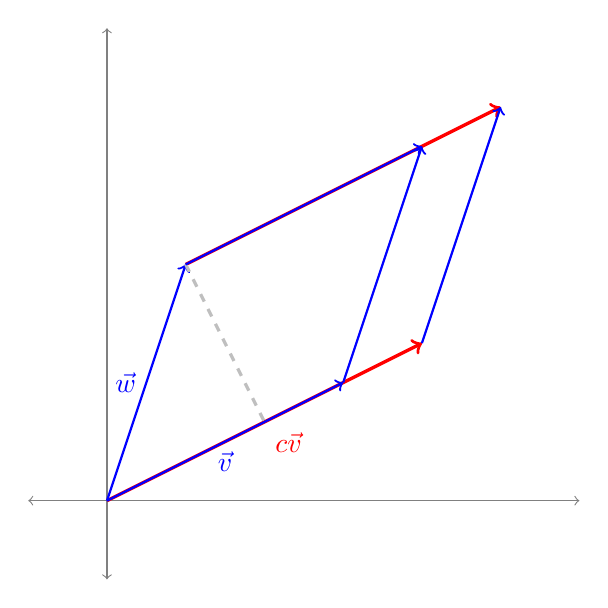
\begin{tikzpicture}
\draw[thin,gray,<->] (-1,0)-- (6,0);
\draw[thin,gray,<->] (0,-1)-- (0,6);
\draw[very thick,red,->] (0,0) -- node[below right] {$c\vec{v}$}  (4,2);
\draw[very thick,red,->] (1,3) -- (5,5);
\draw[thick,blue,->] (0,0) -- node[below] {$\vec{v}$} (3,1.5);
\draw[thick,blue,->] (0,0) -- node[left] {$\vec{w}$} (1,3);
\draw[lightgray,very thick,dashed] (1,3) -- (2,1);
\draw[thick,blue,->] (3,1.5) -- (4,4.5);
\draw[thick,blue,->] (1,3) -- (4,4.5);


\draw[thick,blue,->] (4,2) -- (5,5);
\end{tikzpicture}
\end{center}
  \begin{enumerate}[a)]
    \item $\det([\vec{v}\hspace{0.5em} \vec{w}])=\det([c\vec{v}\hspace{0.5em} \vec{w}])$
    \item $c+\det([\vec{v}\hspace{0.5em} \vec{w}])=\det([c\vec{v}\hspace{0.5em} \vec{w}])$
    \item $c\det([\vec{v}\hspace{0.5em} \vec{w}])=\det([c\vec{v}\hspace{0.5em} \vec{w}])$
  \end{enumerate}
\end{activity}

\begin{activity}{5}
The transformations of unit squares by the
standard matrices \([\vec{u}\hspace{0.5em} \vec{w}]\), \([\vec{v}\hspace{0.5em} \vec{w}]\) and
\([\vec{u}+\vec{v}\hspace{0.5em} \vec{w}]\) are illustrated below.
How is $\det([\vec{u}+\vec{v}\hspace{0.5em} \vec{w}])$ related to
$\det([\vec{u}\hspace{0.5em} \vec{w}])$ and $\det([\vec{v}\hspace{0.5em} \vec{w}])$?
\begin{center}
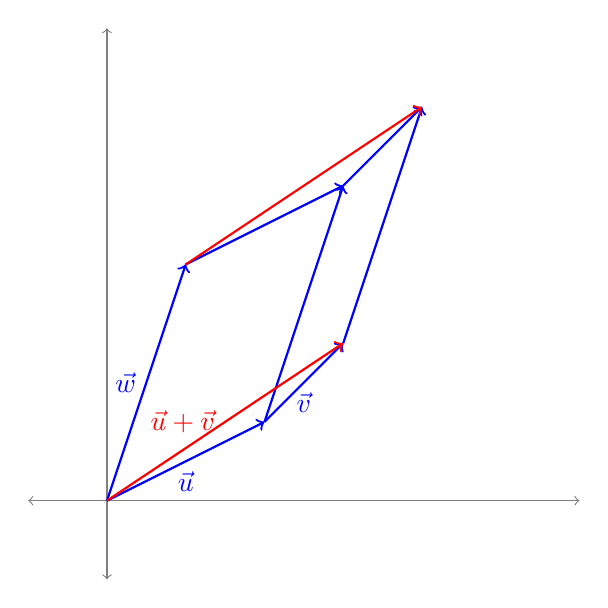
\begin{tikzpicture}
\draw[thin,gray,<->] (-1,0)-- (6,0);
\draw[thin,gray,<->] (0,-1)-- (0,6);
\draw[thick,blue,->] (0,0) -- node[below] {$\vec{u}$} (2,1);
\draw[thick,blue,->] (0,0) -- node[left] {$\vec{w}$} (1,3);
\draw[thick,blue,->] (2,1) -- node [below] {$\vec{v}$}(3,2);
\draw[thick,blue,->] (2,1) -- (3,4);
\draw[thick,blue,->] (3,2) -- (4,5);
\draw[thick,blue,->] (1,3) -- (3,4);
\draw[thick,blue,->] (3,4) -- (4,5);
\draw[thick,red,->] (0,0) -- node[above,left] {$\vec{u}+\vec{v}$} (3,2);
\draw[thick,red,->] (1,3) -- (4,5);
\end{tikzpicture}
\end{center}
  \begin{enumerate}[a)]
    \item
    $\det([\vec{u}\hspace{0.5em} \vec{w}])=\det([\vec{v}\hspace{0.5em} \vec{w}])=\det([\vec{u}+\vec{v}\hspace{0.5em} \vec{w}])$
    \item
    $\det([\vec{u}\hspace{0.5em} \vec{w}])+\det([\vec{v}\hspace{0.5em} \vec{w}])=\det([\vec{u}+\vec{v}\hspace{0.5em} \vec{w}])$
    \item
    $\det([\vec{u}\hspace{0.5em} \vec{w}])\det([\vec{v}\hspace{0.5em} \vec{w}])=\det([\vec{u}+\vec{v}\hspace{0.5em} \vec{w}])$
  \end{enumerate}
\end{activity}


\begin{definition}
The \term{determinant} is the unique function
\(\det:\IR^{n\times n}\to\IR\) satisfying the following three properties:
\begin{enumerate}
\item [P1:] $\det(I)=1$
\item [P2:] $\det([\vec{v}_1\hspace{0.5em}\vec{v}_2\hspace{0.5em}
\cdots\hspace{0.5em}\vec{v}_n])=0$ whenever two columns of the matrix are identical.
\item[P3:]
\(\det[\cdots\hspace{0.5em}c\vec{v}+d\vec{w}\hspace{0.5em}\cdots]=
c\det[\cdots\hspace{0.5em}\vec{v}\hspace{0.5em}\cdots]+
d\det[\cdots\hspace{0.5em}\vec{w}\hspace{0.5em}\cdots]\), assuming
all other columns are equal.
\end{enumerate}
\end{definition}

% \begin{activity}{5}
% True or false: \(\det([\vec{v}\hspace{0.5em}\vec{v}+\vec{w}]) =
% \det([\vec{v}\hspace{0.5em}\vec{w}])\).
%
% \begin{center}
% \begin{tikzpicture}
% \draw[thin,gray,<->] (-1,0)-- (8,0);
% \draw[thin,gray,<->] (0,-1)-- (0,5);
% \draw[very thick,blue,->] (0,0) -- node[below right] {$\vec{v}$}  (3,1);
% \draw[very thick,blue,->] (0,0) -- node[left] {$\vec{w}$} (1,2);
% \draw[dashed,blue,->] (1,2) -- (4,3);
% \draw[dashed,blue,->] (3,1) -- (4,3);
% \draw[thick,red,->] (0,0) --  (4,3)node[above left] {$\vec{v}+\vec{w}$};
% \draw[dashed,red,->] (3,1) -- (7,4);
% \draw[dashed,red,->] (4,3) -- (7,4);
% \end{tikzpicture}
% \end{center}
% \end{activity}

\begin{observation}
Multiples of columns may be may be added to other
columns without affecting the value of a determinant.
  \begin{align*}
  \det([\vec{v}\hspace{1em}\vec{w}])
&=
  \det([\vec{v}\hspace{1em}\vec{w}])+
  c\cdot 0
\\ &=
  \det([\vec{v}\hspace{1em}\vec{w}])+
  c\det([\vec{w}\hspace{1em}\vec{w}])
\\ &=
  \det([\vec{v}\hspace{1em}\vec{w}])+
  \det([c\vec{w}\hspace{1em}\vec{w}])
\\ &=
  \det([\vec{v}+c\vec{w}\hspace{1em}\vec{w}])
  \end{align*}
\end{observation}

\begin{observation}
Determinants represent a \textit{signed} area, since they are not always
positive. In fact, reversing two columns results in a negation of the
determinant.
  \begin{align*}
  \det([\vec{v}\hspace{1em}\vec{w}])
&=
  \det([\vec{v}+\vec{w}\hspace{1em}\vec{w}])
\\ &=
  \det([\vec{v}+\vec{w}\hspace{1em}\vec{w}-(\vec{v}+\vec{w})])
\\ &=
  \det([\vec{v}+\vec{w}\hspace{1em}-\vec{v}])
\\ &=
  \det([\vec{v}+\vec{w}-\vec{v}\hspace{1em}-\vec{v}])
\\ &=
  \det([\vec{w}\hspace{1em}-\vec{v}])
\\ &=
  -\det([\vec{w}\hspace{1em}\vec{v}])
  \end{align*}
\end{observation}



\begin{fact}
  We've shown that the column versions of the three row-reducing operations
  a matrix may be used to simplify a determinant:
  \begin{enumerate}[(a)]
  \item Multiplying a column by a scalar multiplies the
        determinant by that scalar:
        \[c\det([\vec{v}\hspace{0.5em} \vec{w}])=
        \det([c\vec{v}\hspace{0.5em} \vec{w}])\]
  \item Adding a multiple of a column to another column does not
        change the determinant:
        \[\det([\vec{v}\hspace{1em}\vec{w}])=
        \det([\vec{v}+c\vec{w}\hspace{1em}\vec{w}])\]
  \item Swapping two columns changes the sign of the determinant:
        \[\det([\vec{v}\hspace{1em}\vec{w}])=
        -\det([\vec{w}\hspace{1em}\vec{v}])\]
  \end{enumerate}
\end{fact}

\begin{activity}{5}
  The transformation given by the standard matrix \(A\) scales areas by
  \(4\), and the transformation given by the standard matrix \(B\) scales
  areas by \(3\). How must the transformation given by the standard matrix
  \(AB\) scale areas?
  \begin{enumerate}[(a)]
  \item \(1\)
  \item \(7\)
  \item \(12\)
  \item Cannot be determined
  \end{enumerate}

\end{activity}

\begin{fact}
Since the transformation given by the standard matrix \(AB\) is obtained
by applying the transformations given by \(A\) and \(B\), it follows that \[\det(AB)=\det(A)\det(B)\]
%
% \ \\
%
% In particular, a matrix is invertible if and only if its determinant is nonzero.
\end{fact}


\end{applicationActivities}
